\documentclass[11pt]{article}

\usepackage{graphicx}
\usepackage{courier}
\usepackage{underscore}
\usepackage{listings}
\setcounter{secnumdepth}{4}

\title{TMD to Turing Machine Compilation}
\author{Adam Yedidia}

\begin{document}
    
\maketitle

This document is an explanation of the TMD-to-Turing-machine compilation process. It won't be useful to users who only want to know how to use TMD programs, or how to create their own. Rather, it is intended for an audience who is simply curious about how the compilation process works, or wants to write their own language which will compile down to a Turing machine. \\

\section{Basic Structure}

A directory of TMD functions is converted at compilation time to a string of bits to be written onto the tape, along with other states designed to interpret these bits. \ The resulting Turing machine has three main components, or \emph{submachines}: \\

\begin{enumerate}
\item The \emph{initializer} sets up the basic structure of the variable registers and the function stack.
\item The \emph{printer} writes down the binary string that corresponds to the compiled TMD code.
\item The \emph{processor} interprets the compiled binary, modifying the variable registers and the function stack as necessary.
\end{enumerate}

The Turing machine's control flow proceeds from the initializer to the the printer to the interpreter. \ In other words, initializer states point only to initializer states or to printer states, printer states point only to printer states or to interpreter states, and interpreter states point only to interpreter states or the \texttt{HALT} state. \\

The compilation process centers entirely around what binary string is written onto the tape by the printer. Indeed, the processor is identical and the initializer is nearly identical regardless of what the contents of the TMD program are (the initializer will very slightly based on how many functions and variables appear in the TMD program, and on the contents of the \texttt{initvar} file). In contrast, the printer depends entirely on the TMD program, because its job is to write a binary string that encodes the program onto the tape. \\

For this reason, I will not discuss the workings of the initializer or the processor in this document. In fact, I won't even explain how the printer works (it is not as simple as having one state to write each bit in the binary string). Instead, this document will be solely devoted to the details of the encoding scheme that maps TMD onto a binary string. For an explanation of the workings of the initializer, processor, and printer, see: \\ \\
\texttt{parsimony/src/tm/tm_doc.pdf}

\section{Binary String Encoding}

\subsection{Integer Encodings}

In what follows, there will be references made many times to encodings of positive integers. The encoding uses only \texttt{1}'s and \texttt{E}'s, and works as follows: \\ \\
$1 \leftrightarrow \texttt{E}$ \\
$2 \leftrightarrow \texttt{1}$ \\
$3 \leftrightarrow \texttt{EE}$ \\
$4 \leftrightarrow \texttt{E1}$ \\
$5 \leftrightarrow \texttt{1E}$ \\
$6 \leftrightarrow \texttt{11}$ \\
$7 \leftrightarrow \texttt{EEE}$ \\
$8 \leftrightarrow \texttt{EE1}$ \\
$9 \leftrightarrow \texttt{E1E}$ \\
$10 \leftrightarrow \texttt{E11}$ \\
\dots

\subsection{Symbol Encoding}

In what follows, I will make use of the four-symbol alphabet $\{\texttt{_}, \texttt{1}, \texttt{H}, \texttt{E}\}$. This is just for conveniences' sake; without that, making sense of the mapping from semantic meaning to binary string would be even less intelligible than it already is. Recall that \texttt{_} is the blank symbol, and that the mapping from these symbols to the 2-symbol alphabet is as follows:

\begin{itemize}
\item $\texttt{\_} \leftrightarrow \texttt{aa}$
\item $\texttt{1} \leftrightarrow \texttt{ab}$
\item $\texttt{H} \leftrightarrow \texttt{ba}$
\item $\texttt{E} \leftrightarrow \texttt{bb}$
\end{itemize}

\subsection{Function Preamble}

At the start of a new function, the string ``\texttt{HHE_}'' is written. This makes it possible to distinguish lines of code that are part of one function from lines of code that are part of another. Functions are written onto the tape in the order that they appear in \texttt{functions.tff}.

\subsection{Explicit Tape Commands}

All lines of code begin with \texttt{H} to indicate that a new line of code is beginning. Explicit tape commands are followed by a \texttt{1} to indicate that this line of code is an explicit tape command. Following that is a string of \texttt{1}'s and \texttt{E}'s which encodes which variable is being read and written by the command. (These strings of \texttt{1}'s and \texttt{E}'s encode positive integers, and the positive integer $i$ is referencing the $i^\textrm{th}$ argument to the function.) Following that is a \texttt{_} (to indicate that the encoding of the variable is over). \\

After this beginning sequence of symbols, there are a variety of sequences which encode the ``reactions'' of the explicit tape command--in other words, what the Turing machine must do in response to reading each possible TMD symbol (\texttt{_}, \texttt{1}, or \texttt{E}) off the tape. Each reaction begins with a \texttt{1} to indicate that there is a new reaction to be described. (If there are no more reactions to be described, a \texttt{_} is the next symbol instead.) After that, there is a symbol (\texttt{_}, \texttt{1}, or \texttt{E}) that indicates which TMD symbol this reaction is in response to reading. Next is a symbol (\texttt{_}, \texttt{1}, or \texttt{E}) that indicates what symbol should be written back onto the tape. Following that is a symbol (\texttt{_}, \texttt{1}, or \texttt{E}) that indicates which direction to move the head; \texttt{1} means left, \texttt{E} means right, and \texttt{_} means ``no move.'' Finally, there is either a \texttt{_}, which indicates that the next line of code to be read should be the one that follows, or a sequence of \texttt{1}'s and \texttt{E}'s that encodes a positive integer $i$, indicating that $i^\textrm{th}$ line of code of the function is to be read next, followed by a \texttt{_} indicating the end of the encoding. \\

Reactions are written as above onto the tape until there are none left; then a \texttt{_} is the next symbol.

\subsection{Function Calls}

All lines of code begin with \texttt{H} to indicate that a new line of code is beginning. Function calls are followed by an \texttt{E} to indicate that this line of code is an explicit tape commmand. Following that is a sequence of \texttt{1}'s and \texttt{E}'s that encodes a positive integer $i$, indicating that the function being called is the $i^\textrm{th}$ function in the program (according to the order established by \texttt{functions.tff}) followed by a \texttt{_} indicating the end of the encoding of the number. \\

Then, there is, for each argument in the function call, a sequence of \texttt{1}'s and \texttt{E}'s (followed by a \texttt{_}) encoding a positive integer $i$, indicating that the argument being passed to the function call in is referencing the $i^\texttt{th}$ argument we are \emph{currently} in. This is confusing, so let me clarify this a little bit. If we are currently in function $f$, which has arguments $a$, $b$, and $c$, in that order, then the function call $g(2,3,1)$ will corresponds to calling $g(b,c,a)$. \\

Function arguments are written as above until there are none left, after which a \texttt{_} symbol indicates that there are no more arguments to the function call.

\subsection{Return Statements}

All lines of code begin with \texttt{H} to indicate that a new line of code is beginning. Return statements are followed by a \texttt{_} to indicate that this line of code is a return statement.

\section{Post-processing}

It might not be obvious at this point how it is that each line of code is differentiated from each other line of code; the processor, after all, must read a specific line of code from a specific function by matching a function identifier from the function stack to an identical identifier in the program binary. Similarly, the current line number must be matched to its corresponding line number in the program binary. How does this happen, given that no such identifiers appeared in the encoding described in the previous section? \\

The answer is that some post-processing is done after the printer completes. There are a few states devoted to replacing each occurrence of ``\texttt{HH}'' (indicating the start of a function) with an increasing sequence of integer-encodings (using the standard encoding). In this way each function is given a unique identifier, increasing with order of appearance. A similar approach is used for line numbers; for each different line of code, the occurrences of a single ``\texttt{H}'' (indicating the start of a new line) are replaced with an increasing sequence of integer-encodings. (Naturally, a nwe increasing sequence is used for each new function). \\

The idea of this post-processing is simple; ideally, we would like a binary string that includes these identifiers. However, these identifiers are perfectly predictable, so it would be unparsimonious to just write them onto the tape, because they take up a lot of space. Instead, we write them all at once with a post-processing submachine that contains only a constant number of states. This suggests a more general idea: the actual binary string written by the printer, while generally reasonably high-entropy, is certainly not perfectly unpredictable. In theory, as programs get longer and longer, it would be more parsimonious to write a perfectly compressed version of the program binary onto the tape using the printer, and then use ``post-processing'' to decompress the binary, using only a constant-size decompression machine. This is possibly an area for future research; it may not be worth it for programs of the size we've seen so far, but it will be worth it for programs large enough.

\section{Example}

As an example, take the following TMD program: \\ \\ 
\texttt{f.tmd}:
{ \scriptsize \tt
\begin{lstlisting}
input a b c

// Recursively writes a 1 on every tape.

function g a 
[b] 1 (RETURN); E ()
function f b c a
RETURN: return
\end{lstlisting}
}
\texttt{g.tmd}:
{ \scriptsize \tt
\begin{lstlisting}
input x

// Writes a 1 on the input tape.

[x] E (1)
return
\end{lstlisting}
}

\texttt{functions}:
../busybeaver/functions.tex
\texttt{initvar}:
{ \scriptsize \tt
\begin{lstlisting}
E
\end{lstlisting}
}

This program can also be found at: \\ \\
\texttt{parsimony/tmd/tmd_dirs/example_tmd_dir/} \\

This program compiles to the binary string: \\ \\
\texttt{HHE_HE1_E__H11_111_E1_1EE___HEE_1_EE_E__H_HHE_H1E_1E1___H_} \\ 

The breakdown of tape symbols to semantic meaning is shown in Figure~\ref{fig:postprog}.

\begin{figure}
\begin{center}
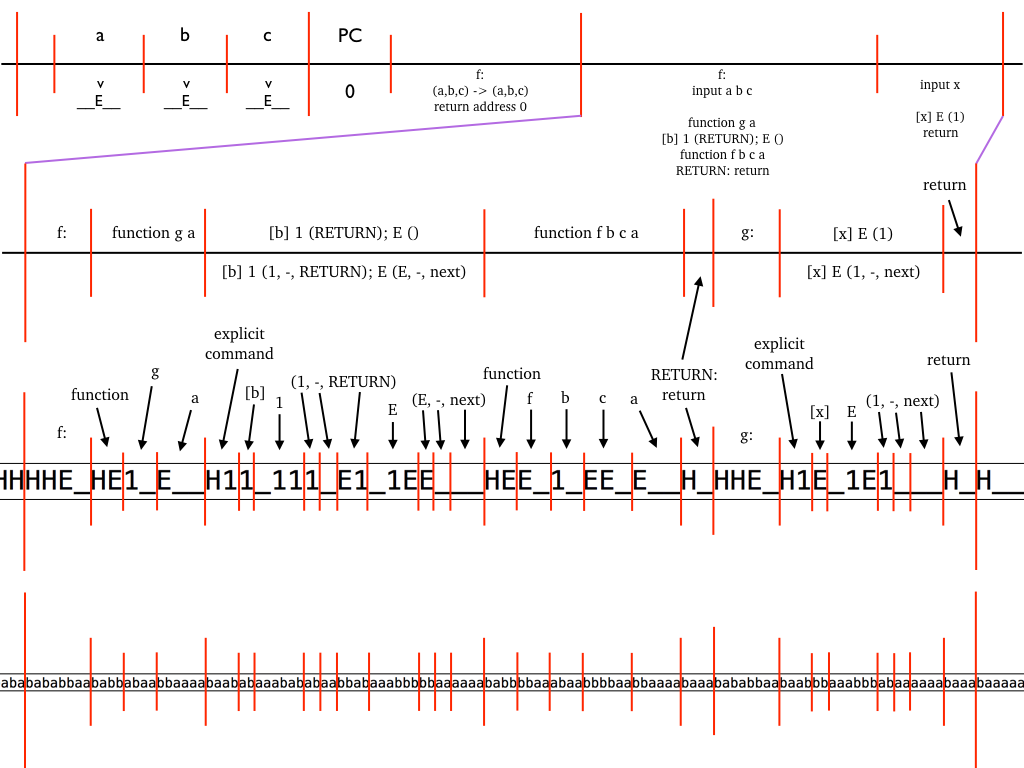
\includegraphics[scale=0.42]{figs/postprog.png}
\caption{The state of the Turing machine tape after the printer completes. \ The top bar is a high-level description of the entire tape; unfortunately, at this point there are so many symbols on the tape that it is impossible to see everything at once. \ The bottom three bars show a zoomed-in view of the program binary. \ From the top, the second bar gives a high-level description of what each part of the program binary means; the third bar gives the direct correspondence between $4$-symbol alphabet symbols on the tape and their meaning in TMD; the fourth and final bar gives the translation of the third bar into the $2$-symbol alphabet. \label{fig:postprog}}
\end{center}
\end{figure}


\end{document}
